%!TEX root=paper/paper.tex
\chapter{Reinforcement Learning for Anytime Classification}

\PM{Motivation}
In the previous chapter, running a detector was a very costly action.
In other settings, such as classification problems, we may want to efficiently select a subset of fast features to compute.
For Anytime performance, we should be able to effectively classify any subset of features our policy selects.

%!TEX root=paper/paper.tex
\section{Problem definition}\label{sec:clf_problem}

\begin{mydef} \label{def:clf_problem}
\textbf{The test-time efficient multi-class classification problem} consists of

\begin{itemize}
    \item $N$ instances labeled with one of $K$ labels: ${\mathcal{D} = \{x_n \in \mathcal{X}, y_n \in \mathcal{Y} = \{1, \dots, K\}\}_{n=1}^N}$.
    \item $F$ features $\mathcal{H} = \{h_f : \mathcal{X} \mapsto \mathbb{R}^{d_f} \}_{f=1}^F$, with associated costs $c_f$.
    \item Budget-sensitive loss $\mathcal{L}_\mathcal{B}$, composed of cost budget $\mathcal{B}$ and loss function ${\ell(\hat{y}, y) \mapsto \mathbb{R}}$.
\end{itemize}

The goal is to find a \textbf{feature selection} policy $\pi(x): \mathcal{X} \mapsto 2^\mathcal{H}$ and a \textbf{feature combination} classifier $g(\mathcal{H}_\pi) : 2^\mathcal{H} \mapsto \mathcal{Y}$ such that such that the total budget-sensitive loss $\sum \mathcal{L}_\mathcal{B}(g(\pi(x_n)), y_n)$ is minimized.
\end{mydef}

\PM{Budget}
The cost of a selected feature subset $\mathcal{H}_{\pi(x)}$ is $C_{\mathcal{H}_\pi(x)}$.
The budget-sensitive loss $\mathcal{L}_\mathcal{B}$ presents a hard budget constraint by only accepting answers with $C_{\mathcal{H}} \leq \mathcal{B}$.
Additionally, $\mathcal{L}_\mathcal{B}$ can be \textbf{cost-sensitive}: answers given with less cost are more valuable than costlier answers.
As discussed in \autoref{sec:introduction}, the motivation for the latter property is Anytime performance; we should be able to stop our algorithm's execution at any time and have the best possible answer.

\PM{Cost}
Feature costs $c_f$ can be specified flexibly, with options including theoretical analysis, number of flops, wall clock runtime, total CPU time, or exact power expenditure.
We believe that a deployment in a modern datacenter is most likely to optimize for power expenditure.
In the absence of reliable ways to measure power, we use total CPU time to define the cost: if an operation is performed in parallel on multiple cores, its cost is considered to be the total cpu time on all cores.

\PM{Shared features}
The features $h_f$ can be classifier outputs, possibly multi-class; following convention, we refer to such features as \emph{weak learners}.
For a weak learner $h_f$, the cost $c_f$ is composed of the cost of an underlying feature extraction $\phi_{h_f}(x)$ and the cost of subsequent classification.
Once $h_f$ is computed, its underlying feature $\phi$ is considered to be free for all other features $h_f'$ that share it, if any, such that $c_f' < c_f$.
Note that in state-of-the-art object recognition systems, complex features and feature encodings are often followed by linear classifiers, and feature extraction cost dominates the total cost.

\begin{figure}[ht]
\centering
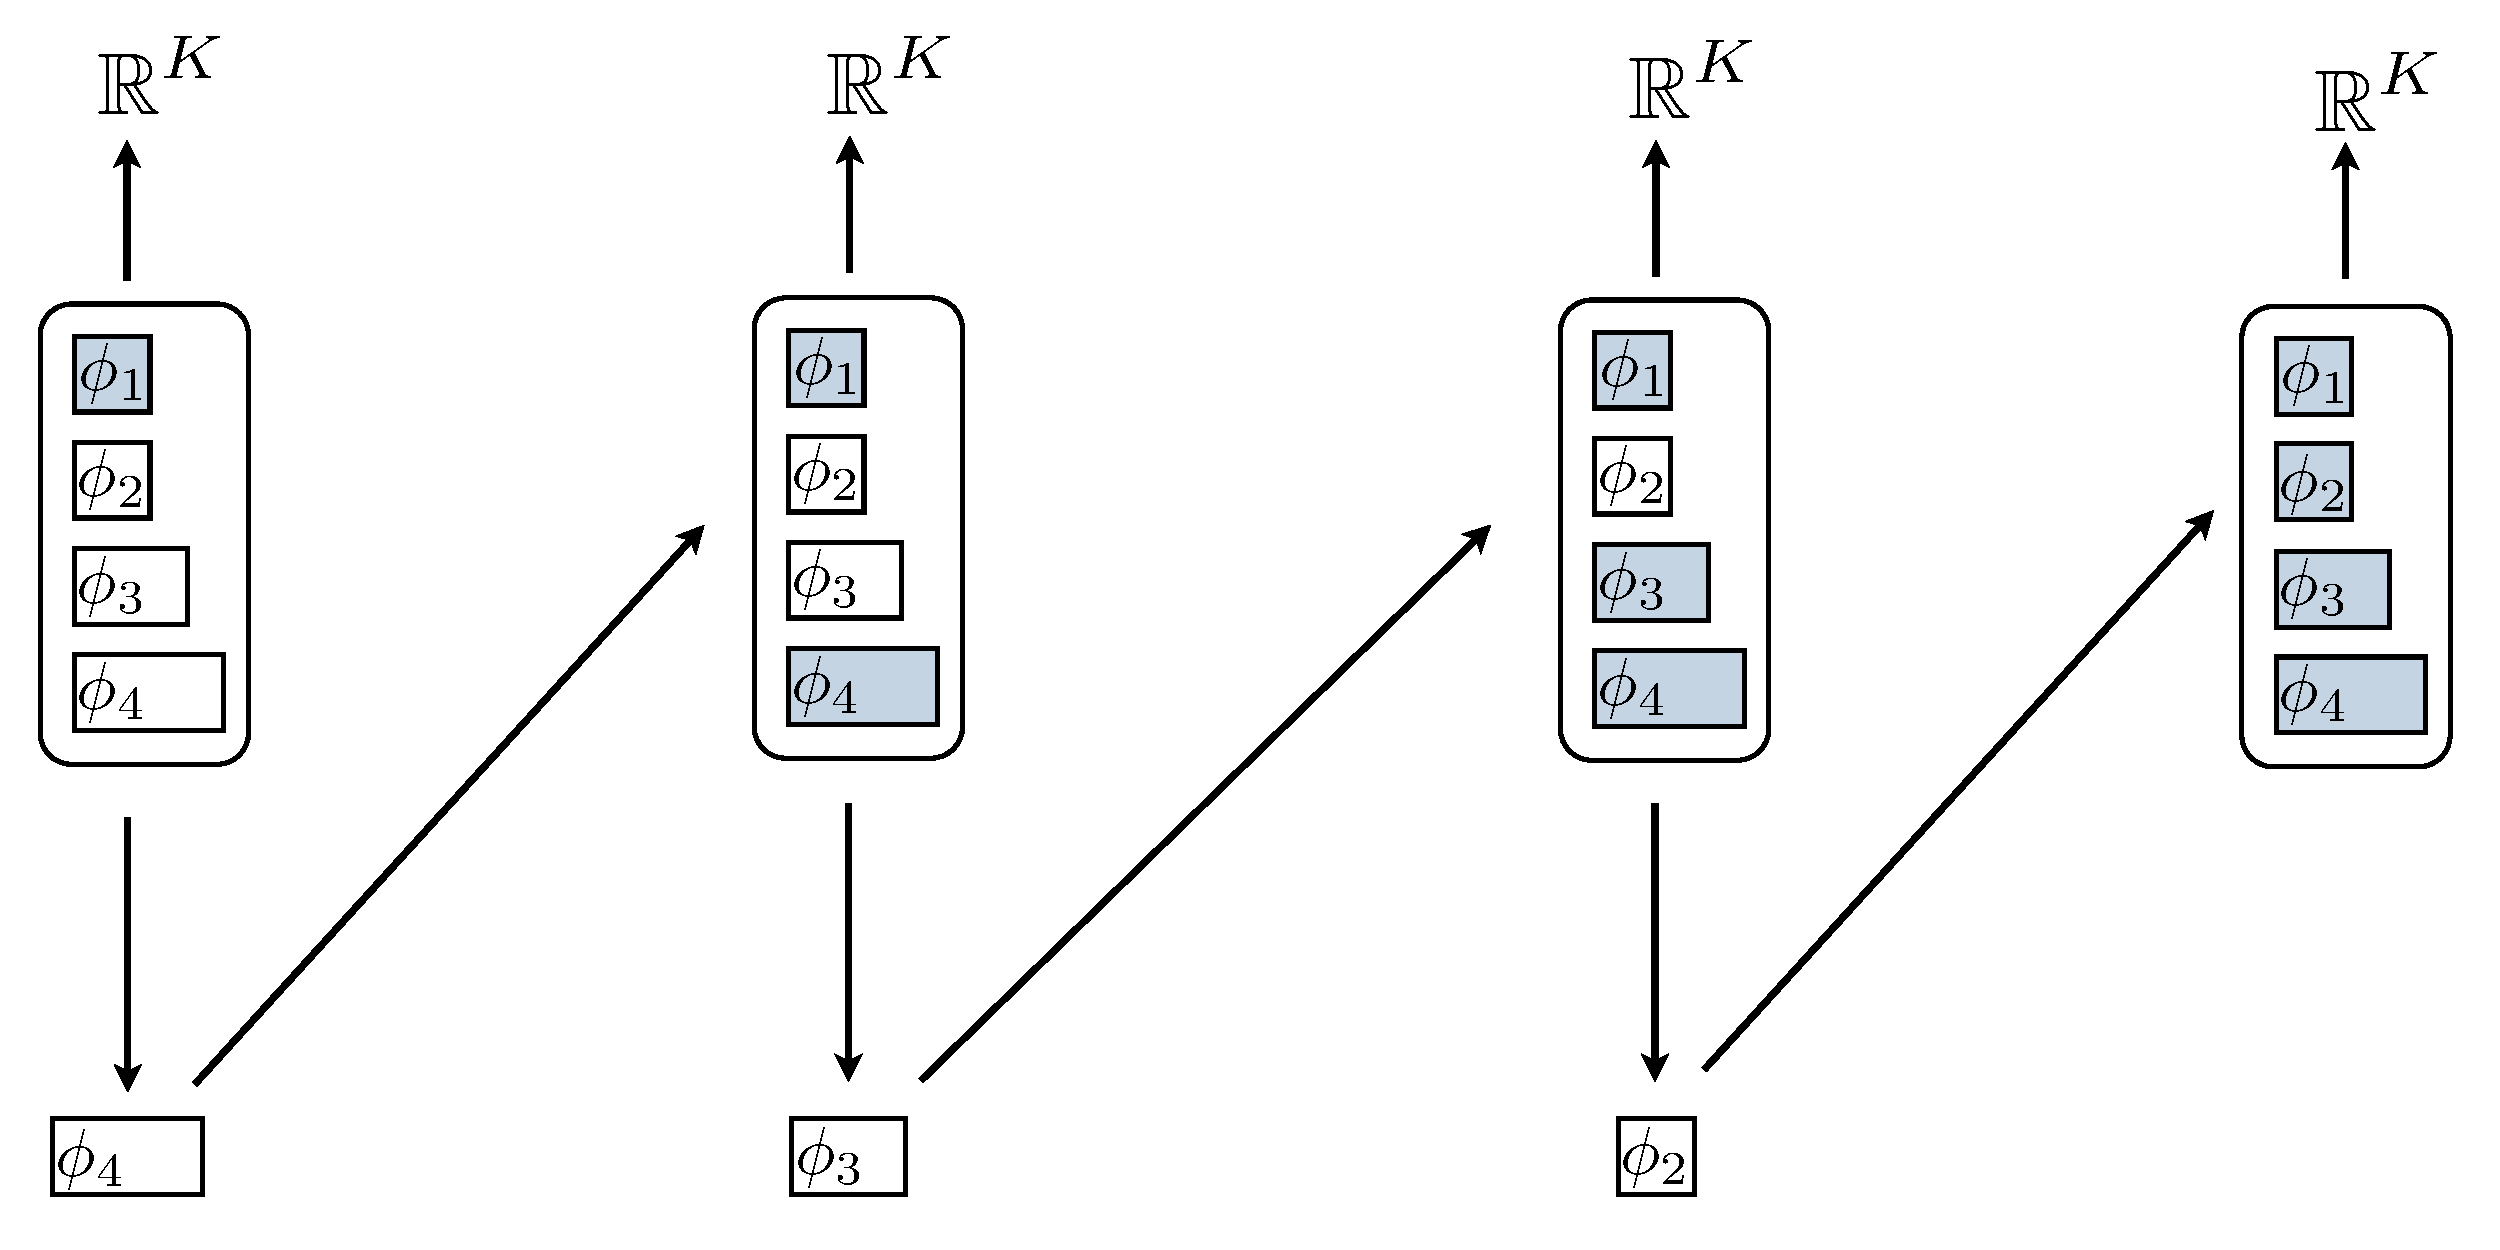
\includegraphics[width=.85\linewidth]{../../figures/feature_selection_sequence.pdf}
\caption[
Summary of our dynamic feature selection approach to the classification problem.]{
We model the problem of state traversal as a Markov Decision Process.
For every state, we learn to select action of maximum expected value.
The state is updated with the result of the selected action.
We train a classifier on subsets of features, to give answer at any time.
}\label{fig:feature_selection_sequence}
\end{figure}


\PM{Train vs. test}
At training time, our computation is unbudgeted, and we can compute all features to have \emph{fully-observed} training instances.
At test time, there is a budget and so the instances we classify will only be \emph{partially-observed}, as determined by the feature selection policy.
\autoref{fig:feature_selection_sequence} shows the sequential process we are learning.


%!TEX root=paper/paper.tex
\section{Method}\label{sec:clf_method}

\PM{MDP}
We model the \textbf{feature selection} policy $\pi(x): \mathcal{X} \mapsto 2^\mathcal{A}$ following the reinforcement learning approach as described in \autoref{sec:mdp_formulation}.
The set of \textbf{actions} $\mathcal{A}$ is exactly the set of features $\mathcal{H}$.
The policy learning approach remains the same, including implementation details.
Three things are different: the reward definition, the state featurization function, and the additional dependence on a classifier.

\PM{Classifier}
We defer discussion of learning the \textbf{feature combination} classifier $g(\mathcal{H}_\pi) : 2^\mathcal{H} \mapsto \mathcal{Y}$ to~\autoref{sec:clf_classifier}.
For now, we assume that $g$ can combine an arbitrary subset of features and provide a distribution $P(Y = y)$.
For example, $g$ could be a Naive Bayes (NB) model trained on the fully-observed data.

%!TEX root=paper/thesis.tex
\subsection{Reward definition}\label{sec:clf_reward}

\begin{figure}[ht]
\centering
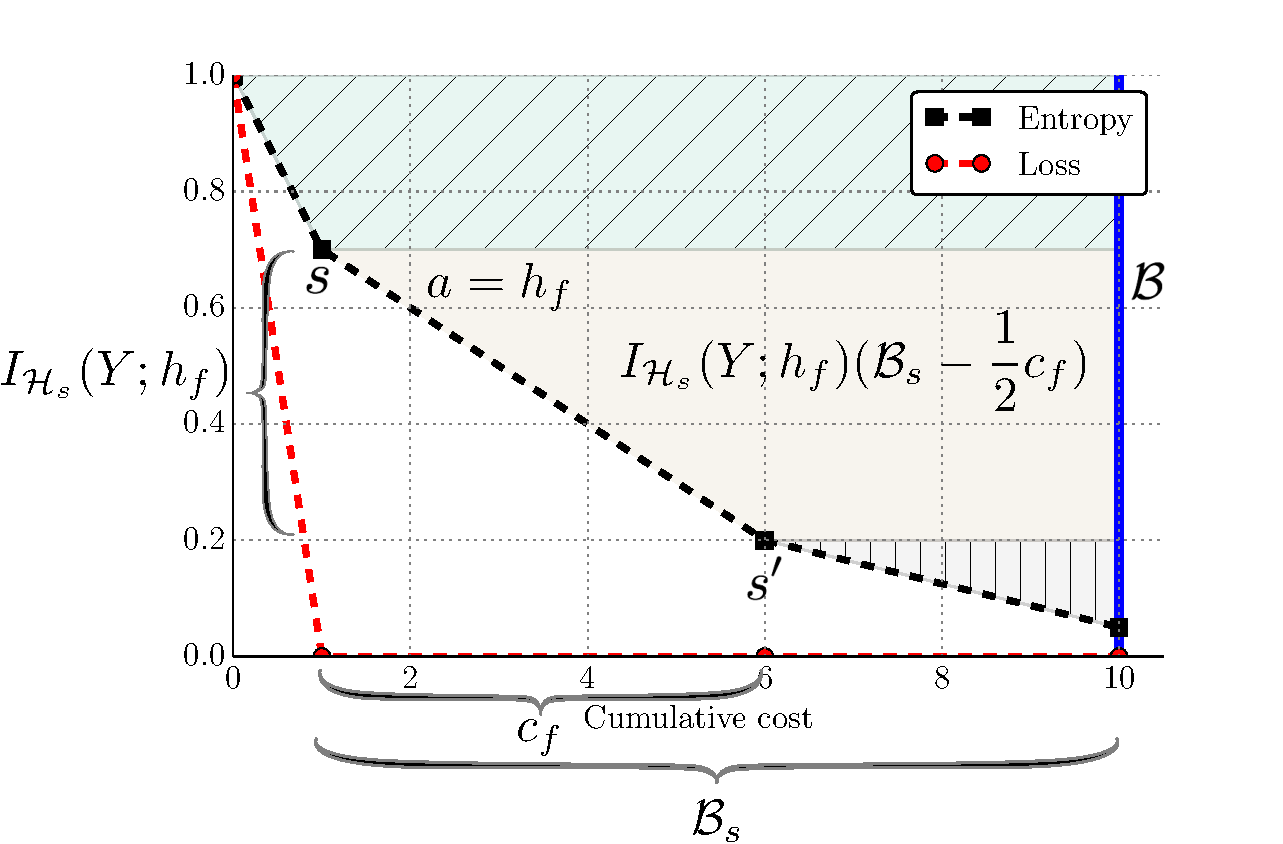
\includegraphics[width=.8\linewidth]{../../figures/rewards.pdf}
\caption{
Definition of the reward function.
To maximize the total area above the entropy vs. cost curve from $0$ to $\mathcal{B}$, we define the reward of an individual action as the area of the slice of the total area that it contributes.
From state $s$, action $a = h_f$ leads to state $s'$ with cost $c_f$.
The information gain is $I_{\mathcal{H}_s}(Y; h_f) = H(Y; \mathcal{H}_s) - H(Y; \mathcal{H}_s \cup {h_f})$.
\label{fig:clf_rewards}}
\end{figure}


\PM{Loss vs. cost}
The budget-sensitive loss $\mathcal{L}_\mathcal{B}$ enforces Anytime performance by valuing early gains more than later gains.
To formalize this, consider \hyperref[fig:clf_rewards]{Figure~\ref*{fig:clf_rewards}}, which shows the entropy and the 0-1 loss of $g$ at every point in a sequential feature selection episode for some instance $x$.
For the best Anytime performance, we want to capture the most area above the loss vs. cost curve, up to max budget $\mathcal{B}$ \parencite{Karayev-NIPS-2012}.
Recall from \eqref{eq:expected_reward} that the value of an episode $\xi$ is defined as the sum of obtained rewards.
If the reward of a single action is defined as the area above the curve that is captured as a direct result, then the value of the whole episode exactly corresponds to $\mathcal{L}_\mathcal{B}$.

\PM{Infogain}
However, there is a problem with using loss directly: only the first action to ``tip the scale'' toward the correct prediction gets a direct reward (in the figure, it is the first action).
A smoother reward function is desirable: if the classifier $g$ can give a full distribution $P(Y = y \mid \mathcal{H}_{\pi(x)})$ and not just a prediction $\hat{y} \in \mathcal{Y}$, we can maximize the \emph{information gain} of the selected subset instead of directly minimizing the loss of $g(\pi(x))$:
\begin{eqnarray}
I(Y; \mathcal{H}_{\pi(x)}) &=& H(Y) - H(Y | \mathcal{H}_{\pi(x)}) = \\ \notag
&=& \sum_{y \in Y} P(y) \log P(y) - \\ \notag
&&\sum_{y, \mathcal{H}_{\pi(x)}} P(y, \mathcal{H}_{\pi(x)}) \log P(y \mid \mathcal{H}_{\pi(x)})
\end{eqnarray}

\PM{Definition}
To the extent that $g$ is unbiased, maximizing information gain corresponds to minimizing loss, and ensures that we not only make the right classification decision but also become maximally certain.
Therefore, as graphically presented in \hyperref[fig:clf_rewards]{Figure~\ref*{fig:clf_rewards}}, we define the reward of selecting feature $h_s$ with cost $c_f$ with the set $\mathcal{H}_s$ computed to be $I_{\mathcal{H}_s}(Y; h_f) (\mathcal{B}_s - \frac{1}{2}c_f)$.
Although we do not evaluate in this regime, note that this definition easily incorporates a \textbf{setup cost} in addition to \textbf{deadline cost} by only computing the area in between setup and deadline costs.


%!TEX root=paper/paper.tex
\subsection{Features of the state}\label{sec:clf_features}

The featurization function $\phi(s)$ extracts the following features from the state:

\begin{itemize}\addtolength{\itemsep}{-.5\baselineskip}
\item Bit vector $\textbf{m}$ of length $F$: initially all bits are $1$ and are set to $0$ when the corresponding feature is computed.
\item For each $h_f$, a vector of size $d_f$ representing the values; $0$ until observed.
\item Cost feature $c \in [0, 1]$, for fraction of the budget spent.
\item Bias feature $1$.
\end{itemize}

\PM{Static vs Dynamic}
These features define the \textbf{dynamic} state, presenting enough information to have a \emph{closed-loop} (dynamic) policy that may select different features for different test instances.
The \textbf{static} state has all of the above features except for the observed feature values.
This enables only an \emph{open-loop} (static) policy, which is exactly the same for all instances.
Policy learned with the static state is used as a baseline in experiments.


\subsection{Learning the classifier.}\label{sec:classifier}

We have so far assumed that $g$ can combine an arbitrary subset of features and provide a distribution $P(Y = y)$---for example, a Gaussian Naive Bayes (NB) model trained on the fully-observed data.
However, a Naive Bayes classifier suffers from its restrictive independence assumptions.

Since discriminative classifiers commonly provide better performance, we use a \textbf{logistic regression} classifier, which presents a new challenge: at test time, some feature values are missing and need to be imputed.

If the classifier is trained exclusively on fully-observed data, then the feature value statistics at test time will not match, resulting in poor performance.
Therefore, we need to learn classifier weights on a distribution of data that exhibits the pattern of missing features induces by the policy $\pi$.
At the same time, learning the policy depends on the classifier $g$, used in the computation of the rewards.

\begin{algorithm}[]
\SetKwFunction{ComputeRewards}{ComputeRewards}
\SetKwFunction{GatherSamples}{GatherSamples}
\SetKwFunction{UpdatePolicy}{UpdatePolicy}
\SetKwFunction{UpdateClassifier}{UpdateClassifier}

\SetAlgoLined
\KwIn{$\mathcal{D} = \{x_n, y_n\}_{n=1}^N$; $\mathcal{L}_\mathcal{B}$}
\KwResult{Trained $\pi$, $g$}
\BlankLine
$\pi_0 \leftarrow$ random\;
\For {$i \leftarrow 1$ \KwTo max\_iterations} {
    States, Actions, Costs, Labels $\leftarrow$ \GatherSamples{$\mathcal{D}$, $\pi_{i-1}$}\;
    $g_i \leftarrow$ \UpdateClassifier{States, Labels}\;
    Rewards $\leftarrow$ \ComputeRewards{States, Costs, Labels, $g_i, \mathcal{L}_\mathcal{B}, \gamma$}\;
    $\pi_i \leftarrow$ \UpdatePolicy{States, Actions, Rewards}\;
}
\caption{Because reward computation depends on the classifier, and the distribution of states depends on the policy, $g$ and $\pi$ are trained iteratively.\label{alg:learning}}
\end{algorithm}


For this reason, the policy and classifier need to be learned jointly: \autoref{alg:learning} gives the iterative procedure.
In summary, we start from random $\pi$ and $g$, gather a batch of trajectories.
The batch is used to update both $g$ and $\pi$.
Then new trajectories are generated with the updated $\pi$, rewards are computed using the updated $g$, and the process is repeated.
This is a variant of generalized policy iteration \cite{Sutton1998}.

\paragraph{Unobserved value imputation.}
Unlike the Naive Bayes classifier, the logistic regression classifier is not able to use an arbitrary subset of features $\mathcal{H}_\pi$, but instead operates on feature vectors of a fixed size.
To represent the feature vector of a fully observed instance, we write $\mathbf{x} = [h_1(x), \dots, h_f(x)]$.
In case that $\mathcal{H}_\pi \subset \mathcal{H}$, we need to fill in unobserved feature values in the vector.

A basic strategy is \textbf{mean imputation}: filling in with the mean value of the feature:
\begin{align}
\mathbf{x}_\pi = \left[ h_i(x) : \left\{ \begin{array}{rl}
 h_i(x) &\mbox{ if $h_i \in \mathcal{H}_{\pi(x)}$} \\
 \bar{\mathbf{h}}_i &\mbox{ otherwise}
\end{array} \right. \right]
\end{align}

If we assume that $\mathbf{x}$ is distributed according to a multivariate Gaussian $\mathbf{x} \sim \mathcal{N}(\mathbf{0}, \Sigma)$, where $\Sigma$ is the sample covariance $X^T X$ and the data is standardized to have zero mean, then it is possible to do \textbf{Gaussian imputation}.
Given a feature subset $\mathcal{H}_\pi$, we write:
\begin{equation}
\mathbf{x}_\pi = \begin{bmatrix} \mathbf{x}^\text{o}\\  \mathbf{x}^\text{u} \end{bmatrix} \sim \mathcal{N} \left( \mathbf{0}, \begin{bmatrix} \mathbf{A} & \mathbf{C}\\ \mathbf{C}^T & \mathbf{B} \end{bmatrix} \right)
\end{equation}
where $\mathbf{x}^\text{o}$ and $\mathbf{x}^\text{u}$ represent the respectively observed and unobserved parts of the full feature vector $\mathbf{x}$.
%, $\mathbf{A}$ is the covariance matrix of $\mathbf{x}^\text{o}$, $\mathbf{B}$ is the covariance matrix of $\mathbf{x}^\text{u}$, and $C$ is the cross-variance matrix that has as many rows as the size of $\mathbf{x}^\text{o}$ and as many columns as the size of $\mathbf{x}^\text{u}$.
%\parencite{Roweis-gaussian-identities}.
In this case, the distribution over unobserved variables conditioned on the observed variables is given as
$\mathbf{x}^\text{u} \mid \mathbf{x}^\text{o} \sim \mathcal{N} \left( \mathbf{C}^T \mathbf{A}^{-1} \mathbf{x}^\text{o},\, \mathbf{B} - \mathbf{C}^T \mathbf{A}^{-1} \mathbf{C} \right)$.

\paragraph{Learning more than one classifier.}
As illustrated in \hyperref[fig:state_space]{Figure~\ref*{fig:state_space}}, the policy $\pi$ selects some feature subsets more frequently than others.
Instead of learning only one classifier $g$ that must be robust to all observed feature subsets, we can learn several classifiers, one for each of the most frequent subsets.
This is done by maintaining a distribution over encountered feature subsets during training.
For each of the $K$ most frequent subsets, a separate classifier is trained, using data that is closest by Hamming distance on the selected-feature bit vector.

Each classifier is trained with the \textsc{Liblinear} implementation of logistic regression, with $L_2$ regularization parameter K-fold cross-validated at each iteration.

\begin{figure}[ht]
\centering
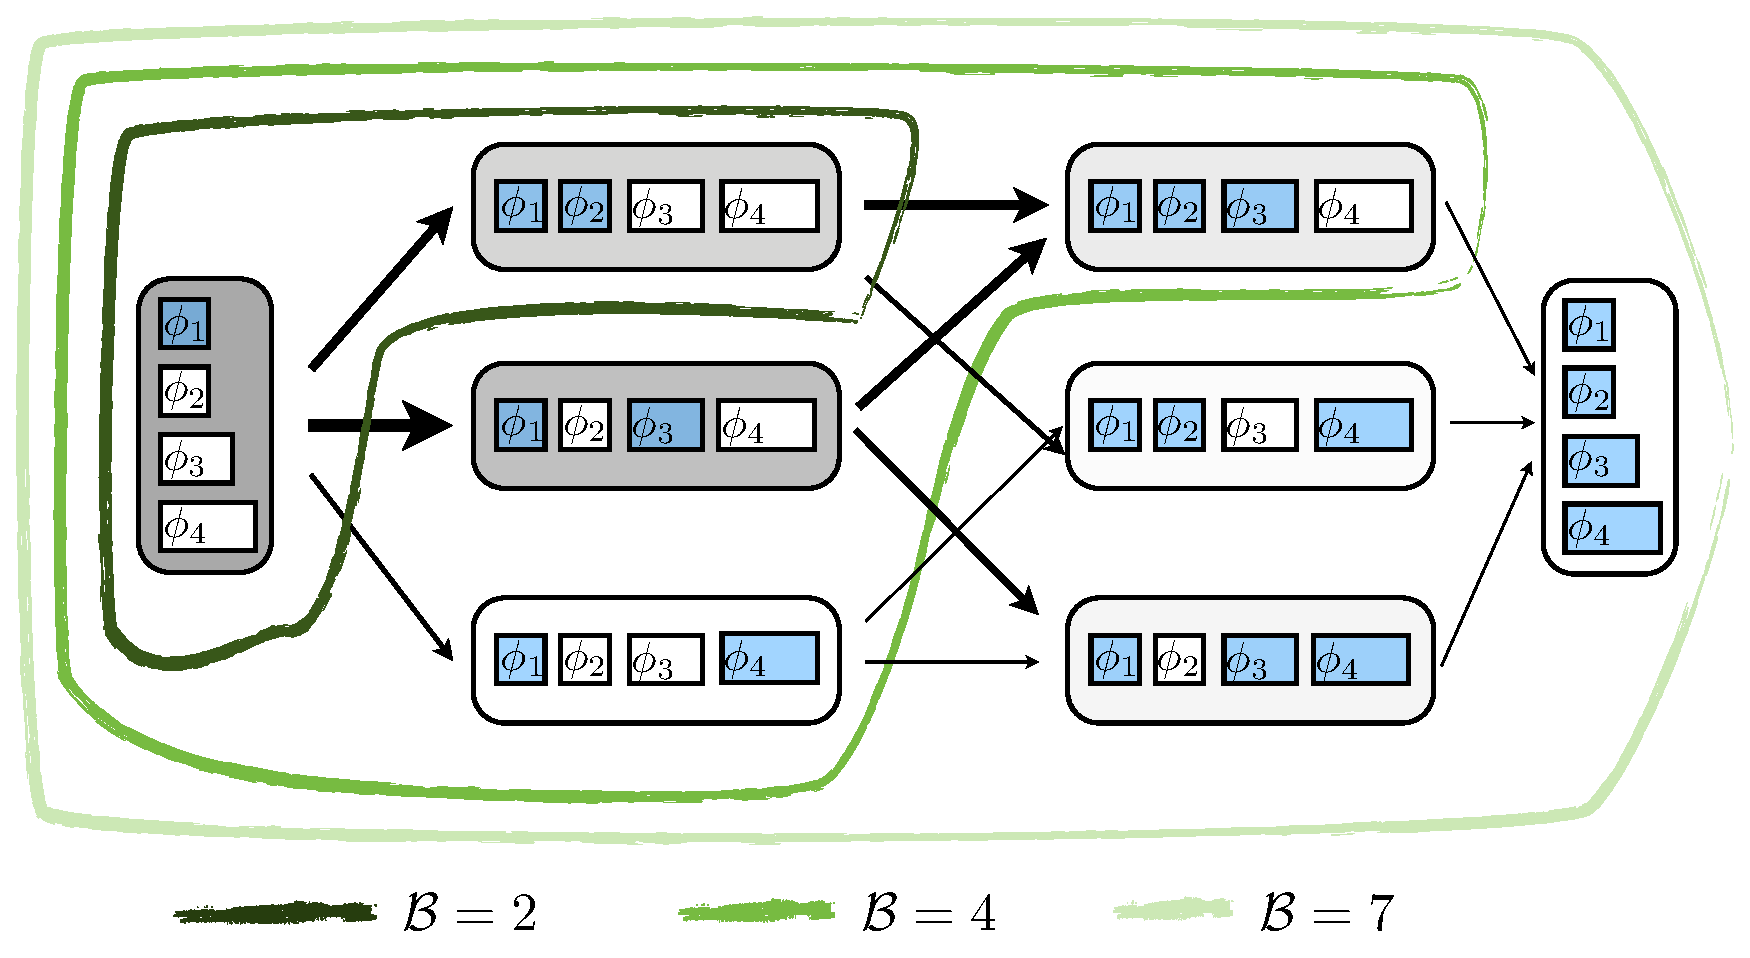
\includegraphics[width=1\linewidth]{../../figures/mdp_masks.pdf}
\caption{
The action space $\mathcal{A}$ of the MDP is the the set of features $\mathcal{H}$, represented by the $\phi$ boxes.
The primary discretization of the state space can be visualized by the possible feature subsets (larger boxes); selected features are colored in the diagram.
The feature selection policy $\pi$ induces a distribution over feature subsets, for a dataset, which is represented by the shading of the larger boxes.
Not all states are reachable for a given budget $\mathcal{B}$.
In the figure, we show three ``budget cuts'' of the state space.
\label{fig:state_space}
}
\end{figure}



%!TEX root=paper/paper.tex
\section{Evaluation}\label{sec:clf_evaluation}

\PM{Settings}
We evaluate the following sequential selection baselines:

\begin{itemize}
\item \textbf{Static, greedy}: corresponds to best performance of a policy that does not observe feature values and selects actions greedily ($\gamma=0$).
\item \textbf{Static, non-myopic}: policy that does not observe feature values but uses the MDP machinery with $\gamma=1$ to consider future action rewards.
\item \textbf{Dynamic, greedy}: policy that observed feature values, but selects actions greedily.
\end{itemize}

Our method is the \textbf{Dynamic, non-myopic} policy: observed feature values, and full lookahead.

\PM{Metrics}
We evaluate two forms of test-time efficient performance measure: the area under the curve and the performance at max budget.
(Note that all methods are trained only for the former measure.)

\PM{Classifier}
In preliminary experiments, Logistic Regression always performed better than the Gaussian Naive Bayes classifier, and so only the former is used in the experiments below.
We evaluated classification with \textbf{Gaussian} vs. \textbf{Mean} imputation, and with different number of classifiers (1, 3, and 6) clustered by feature subsets.
We found that Gaussian imputation performed better than mean imputation, but not substantially, and at additional cost.
Although increased number of classifiers sometimes increased performance, it also made our method prone to overfitting.
In the final accounting, $K=1$ classifiers worked best on all tasks.
Results of detailed experiments on imputation and clustering are given in \autoref{sec:imputation_evaluation}.
For policy experiments, we report only the best achieved imputation method.

\PM{Details}
For details on the reinforcement learning implementation, see \autoref{sec:mdp_formulation} and \autoref{sec:det_evaluation}.
We largely rely on classifier implementations in the \texttt{scikit-learn} package \parencite{Pedregosa2011}.
With pre-computed features, our training procedure takes only a few hours on an $8$-core \emph{Xeon E5620} machine for each of the experiments below.

\subsection{Experiment: Synthetic}

\begin{figure*}[ht]
\centering
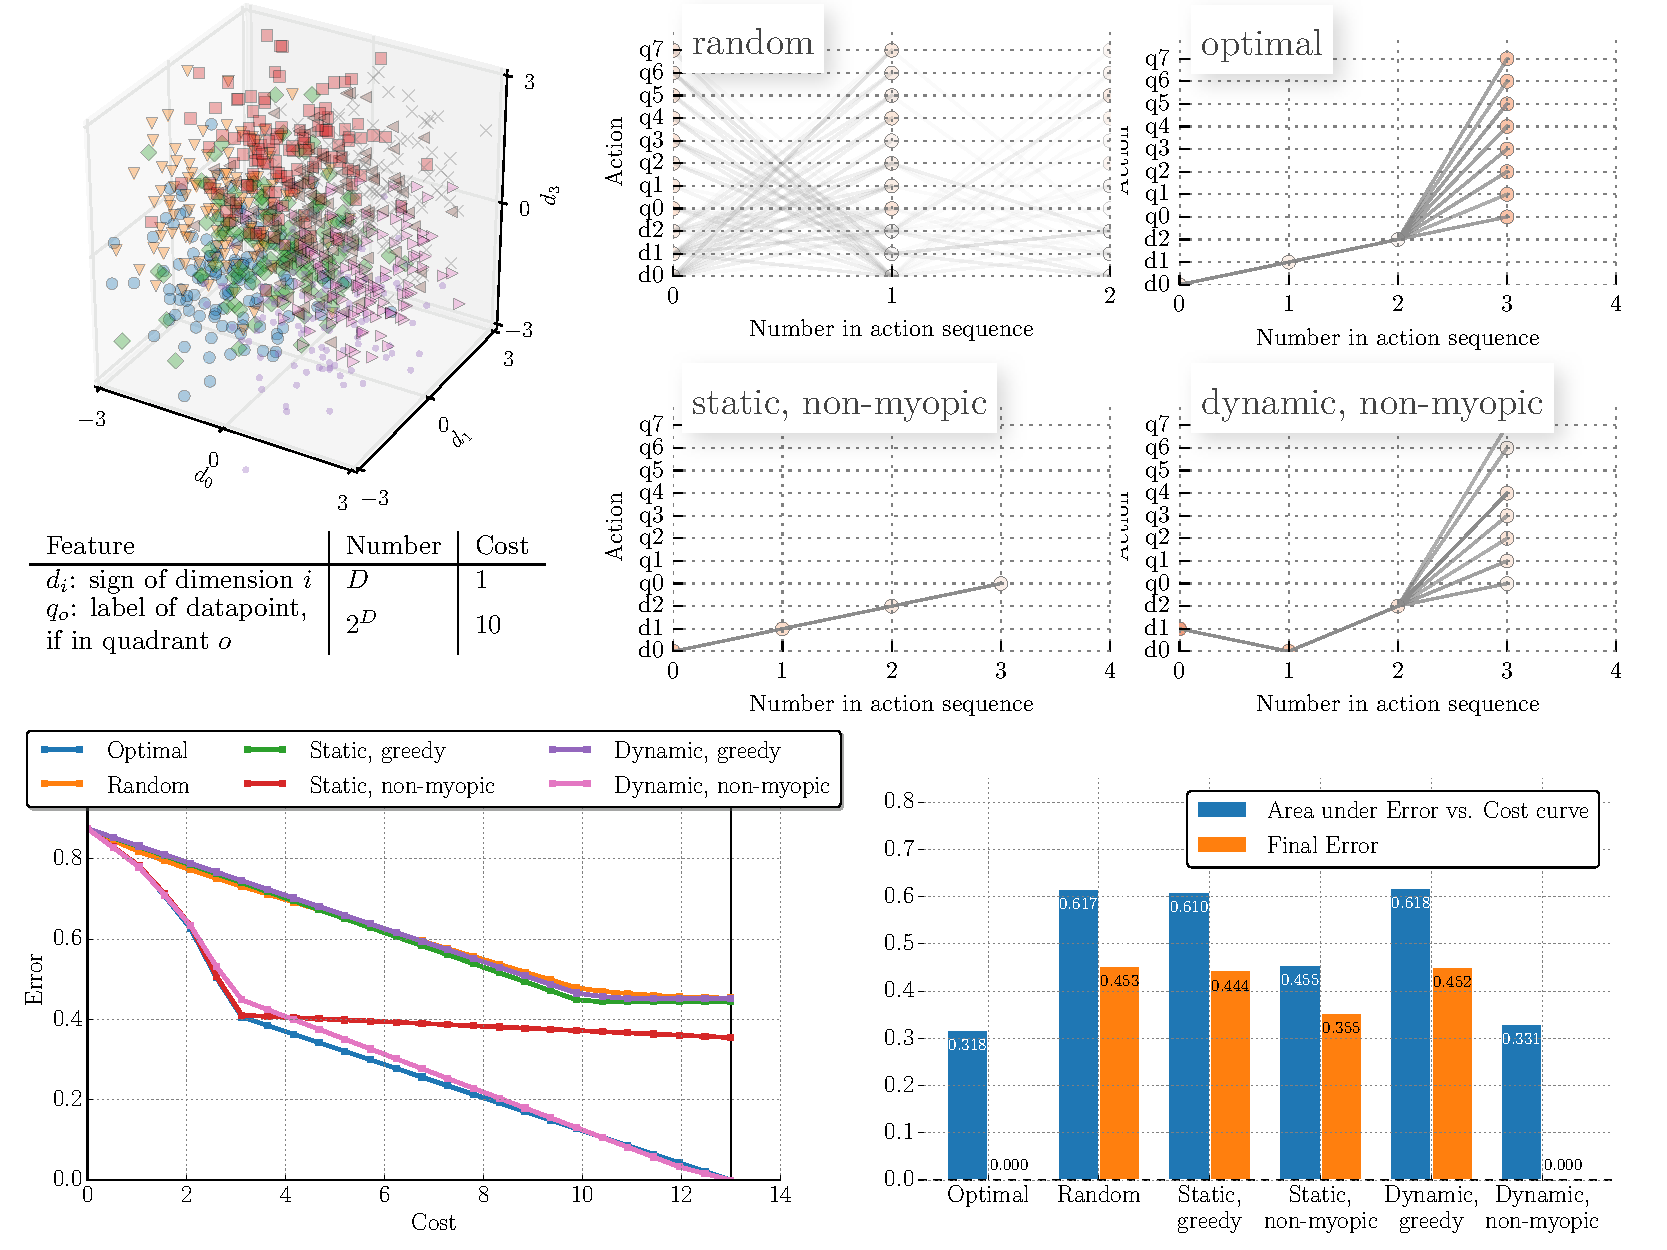
\includegraphics[width=\linewidth]{../../figures/synthetic.pdf}
\caption{
Evaluation on the synthetic example (best viewed in color).
The data and the feature costs are shown at top left; the sample feature trajectories of different policies at top right.
(The opacity of the edges corresponds to their prevalence during policy execution; the opacity of the nodes corresponds to the amount of reward obtained in that state.)
Note that the \emph{static, non-myopic} policy correctly learns to select the cheap features first, but is not able to correctly branch, while our \emph{dynamic, non-myopic} approach finds the optimal strategy.
The plots in the bottom half give the error vs. cost numbers.
}\label{fig:synthetic}
\end{figure*}


\PM{Setup}
Following \cite{Xu-ICML-2013}, we first show that the policy works as advertised in a challenging synthetic example.
In $D$-dimensional space, the data has a label for each of the $2^D$ orthants, and is generated by a unit-variance Gaussian in that orthant (See top left of \autoref{fig:synthetic_setup} for the 3D case).
There are $D$ cheap features that simply return the sign of the data point's coordinate for the corresponding dimension.
For each orthant, there is also an expensive feature that returns the data point's label if the point is located in the corresponding orthant, and random noise otherwise.

\PM{Results}
The optimal policy on a new data point is to determine its orthant with cheap features, and then take the corresponding expensive action.
Note that both dynamic features and non-myopic learning are crucial to the optimal policy, which is successfully found by our approach.
\autoref{fig:synthetic_results} shows the results of this optimal policy, a random policy, and of different baselines and our method, trained given the correct minimal budget.

\subsection{Experiment: Scene recognition}

%!TEX root=paper/paper.tex
\begin{figure*}[ht]
\centering
    \centering
    \begin{subfigure}[b]{0.5\textwidth}
            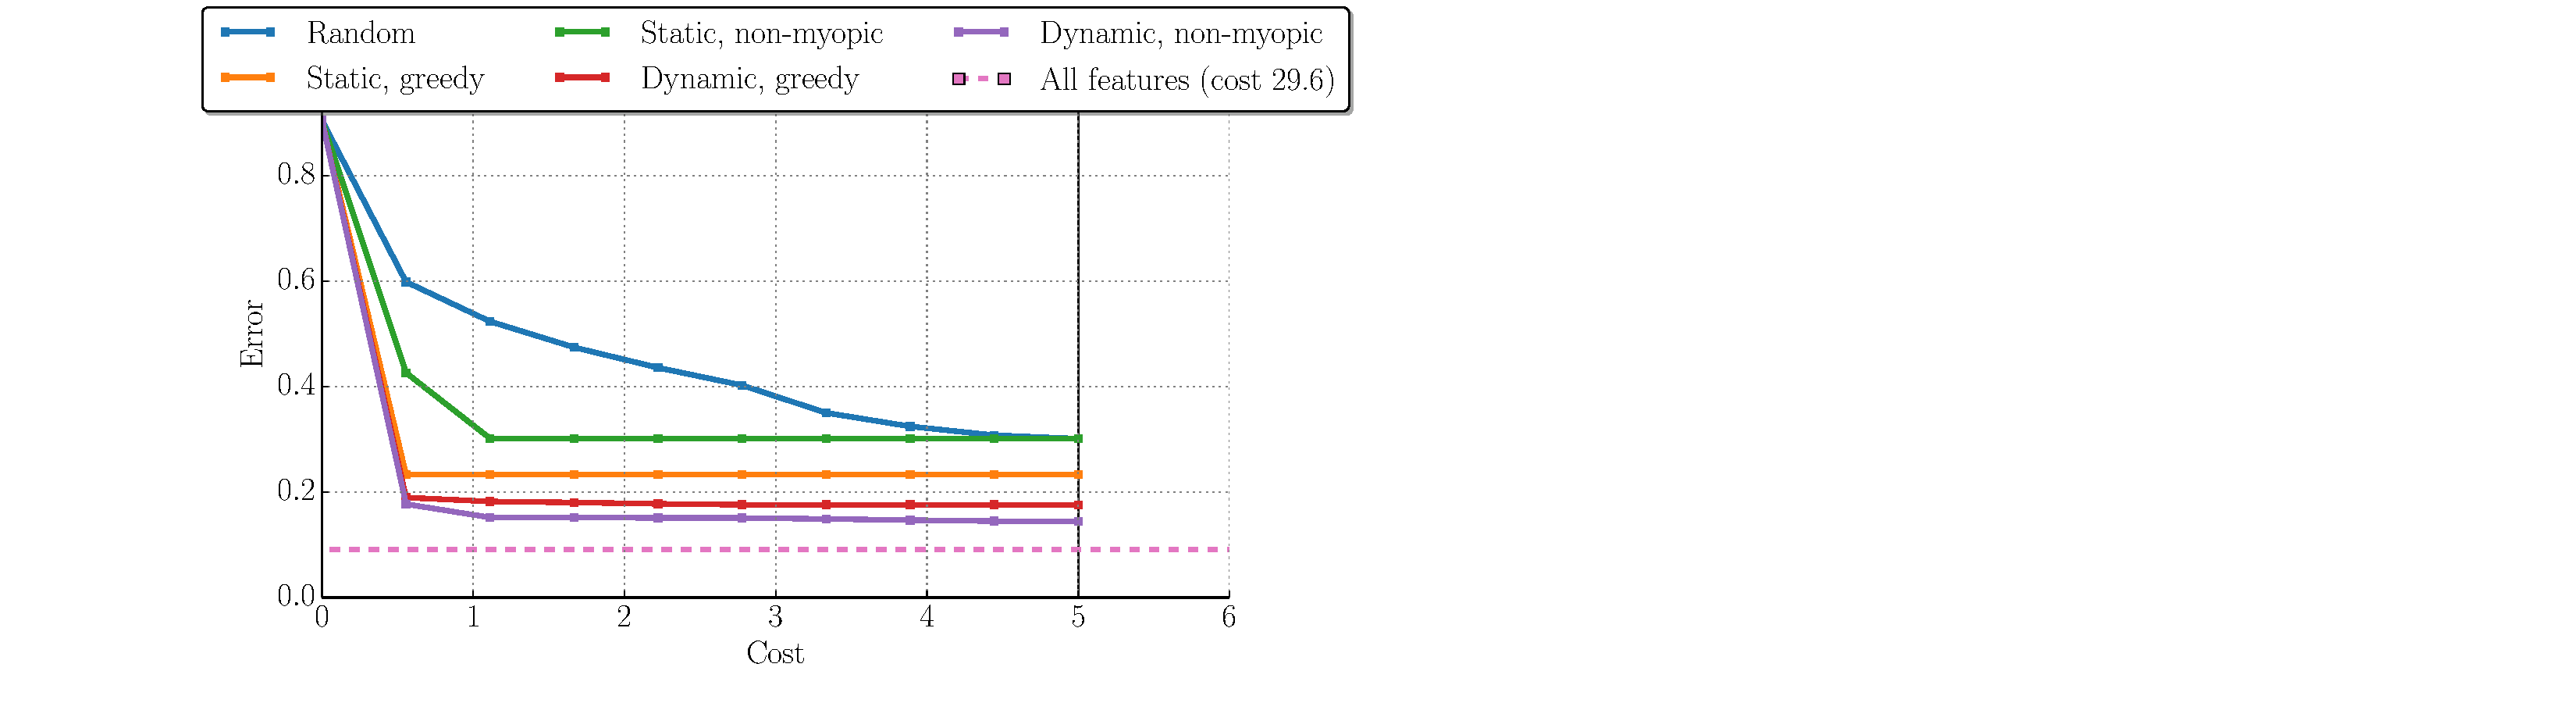
\includegraphics[width=\textwidth]{../../figures/apr11_assembly/scene_15_5_crop.pdf}
            \caption{Error given by policies learned for a budget = 5.}
    \end{subfigure}%
    \begin{subfigure}[b]{0.44\textwidth}
            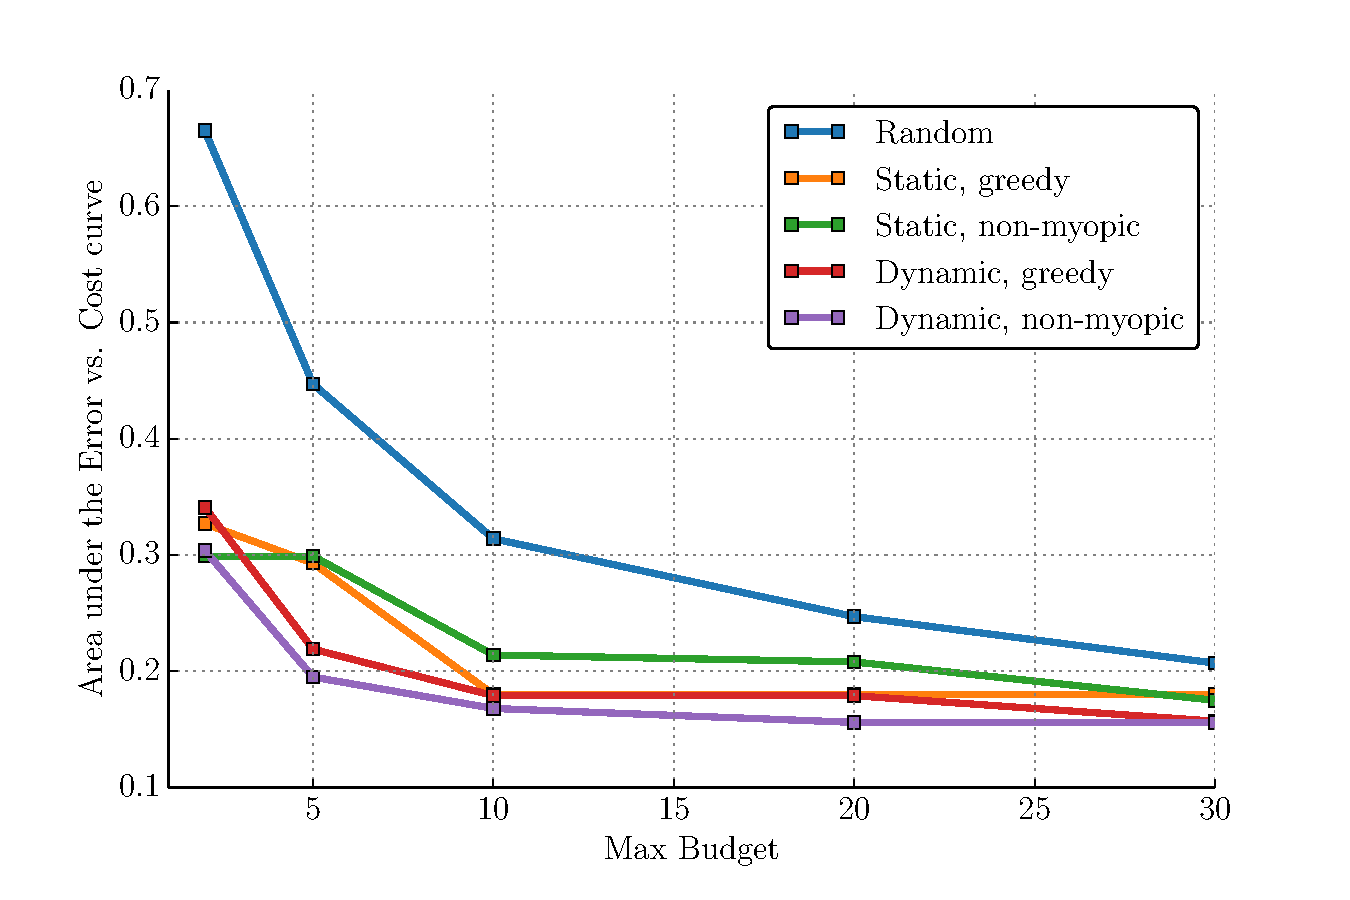
\includegraphics[width=\textwidth]{../../figures/apr11_assembly/_scenes15_auc.pdf}
            \caption{Areas under error vs. cost curves of policies learned at different budgets.}
    \end{subfigure}\\
    \begin{subfigure}[b]{0.47\textwidth}
            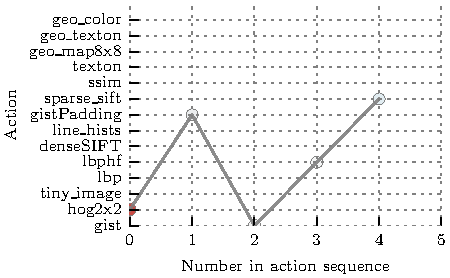
\includegraphics[width=\textwidth]{../../figures/apr11_assembly/scene15_5/static.pdf}
            \caption{Trajectory of our static policy.}
    \end{subfigure}%
    \begin{subfigure}[b]{0.47\textwidth}
            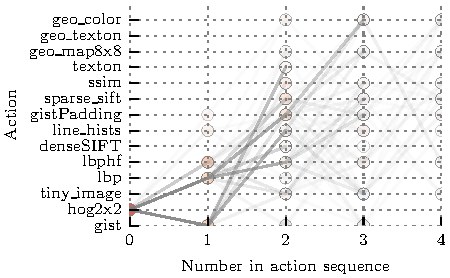
\includegraphics[width=\textwidth]{../../figures/apr11_assembly/scene15_5/dynamic.pdf}
            \caption{Trajectory of our dynamic policy.}
    \end{subfigure}\\
    \caption[Results of the classification approach on the Scenes-15 dataset.]{
Results on Scenes-15 dataset (best viewed in color).
Figure (a) shows the error vs. cost plot for policies learned given a budget of 5 seconds.
Figure (b) aggregates the area under the error vs. cost plot metrics for different policies and budgets, showeing that our approach outperforms baselines no matter what budget it's trained for.
Figures (d) and (e) shows the branching behavior of our dynamic policy vs the best static policy.
}\label{fig:clf_scenes}
\end{figure*}


\PM{Setup}
The Scene-15 dataset \parencite{Lazebnik-CVPR-2006} contains 4485 images from 15 visual scene classes.
The task is to classify images according to scene.
Following \parencite{Xiao-CVPR-2010}, we extracted 14 different visual features (GIST, HOG, TinyImages, LBP, SIFT, Line Histograms, Self-Similarity, Textons, Color Histograms, and variations).
The features vary in cost from 0.3 seconds to 8 seconds, and in single-feature accuracy from 0.32 (TinyImages) to .82 (HOG).
Separate multi-class linear SVMs were trained on each feature channel, using a random 100 positive example images per class for training.
We used the \texttt{liblinear} implementation, and K-fold cross-validated the penalty parameter $C$.
The trained SVMs were evaluated on the images not used for training, resulting in a dataset of 2238 vectors of 210 confidence values: 15 classes for each of the 14 feature channels.
This dataset was split 60-40 into training and test sets for our experiments.

\PM{Results}
\autoref{fig:clf_scenes} shows the results, including learned policy trajectories.
For all evaluated budgets, our \emph{dynamic, non-myopic} method outperforms all others on the area under the error vs. cost curve metric.
Our results on this dataset match the reported results of Active Classification \parencite{Gao-NIPS-2011} (Figure 2) and Greedy Miser \parencite{Xu-ICML-2012} (Figure 3), although both methods use an additional powerful feature channel (ObjectBank)\footnote{Detailed results for this and other experiments are on the project page (see front page for the \href{http://sergeykarayev.com/recognition-on-a-budget/}{link}).}.

\subsection{Experiment: ImageNet and maximizing specificity}

\begin{figure*}[ht]
\centering
    \begin{subfigure}[b]{0.52\textwidth}
            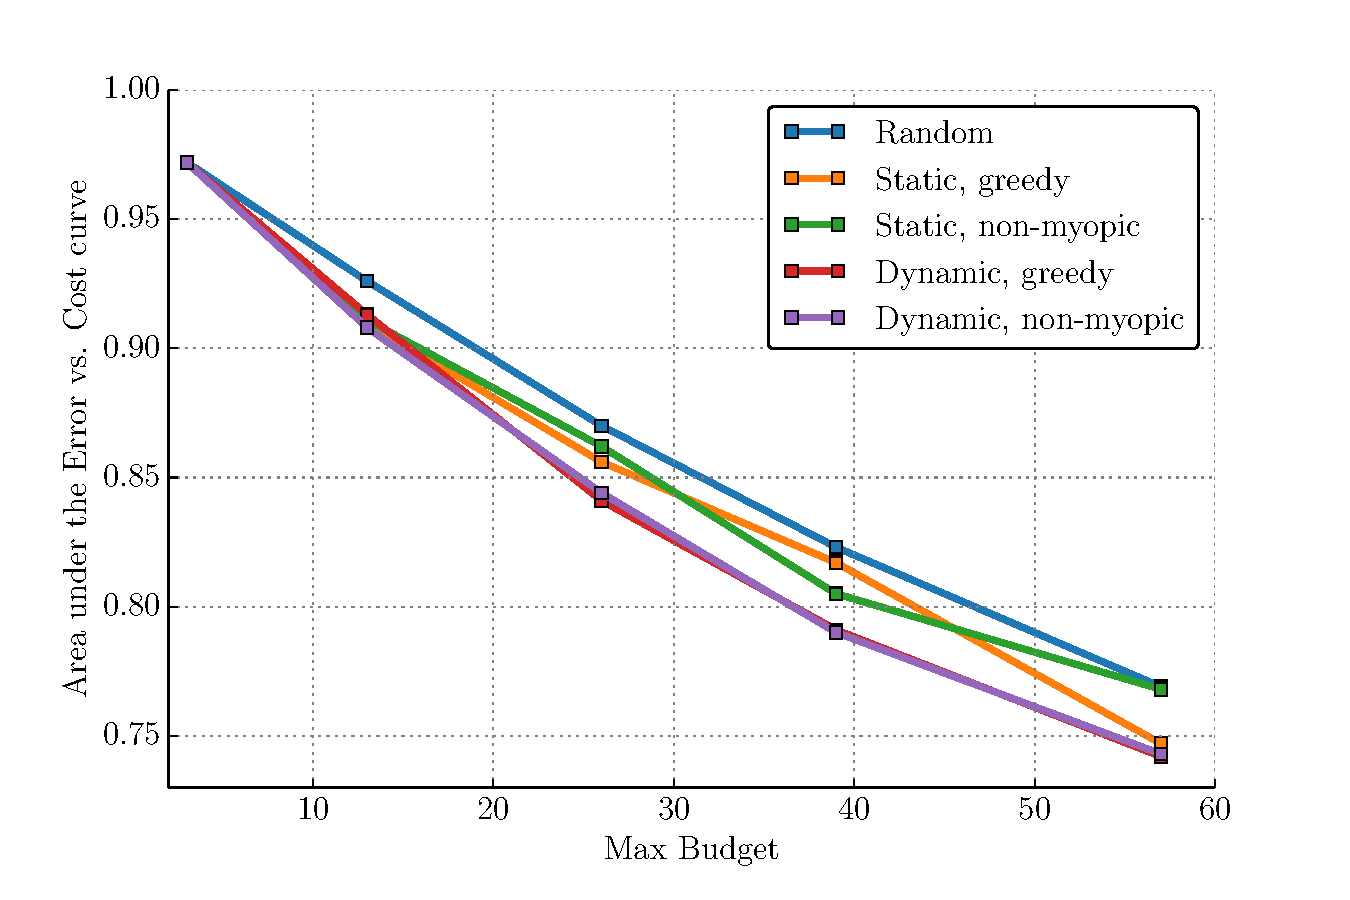
\includegraphics[width=\textwidth]{../../figures/apr11_assembly/_ilsvrc65_auc.pdf}
            \caption{
            Areas under error vs. cost curves for policies learned at different budgets.
            (No specificity back-off is performed here).
            \label{fig:imagenet-a}
            }
    \end{subfigure}\hfill%
    \begin{subfigure}[b]{0.43\textwidth}
            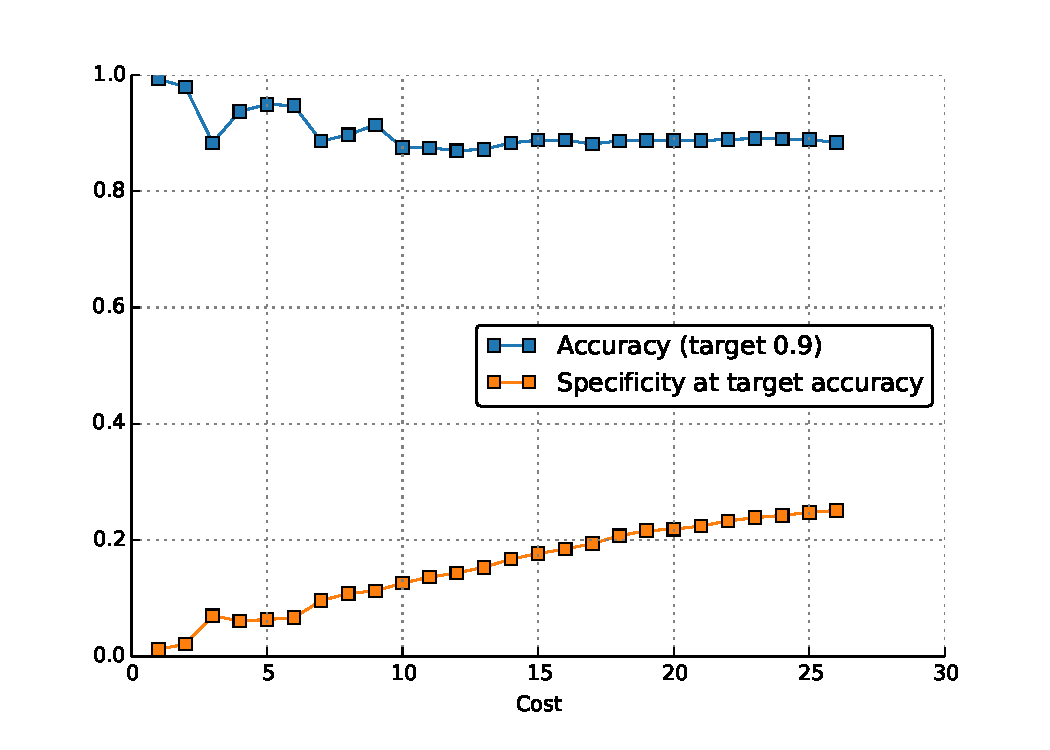
\includegraphics[width=\textwidth]{../../figures/apr11_assembly/ilsvrc65_acc.pdf}
            \caption{
            Holding prediction accuracy constant, we achieve increased specificity with increased cost (on \emph{Dynamic, non-myopic} policy, budget = 36).
            \label{fig:imagenet-b}
            }
    \end{subfigure}\\\vspace{1em}
    \begin{subfigure}[b]{.97\textwidth}
            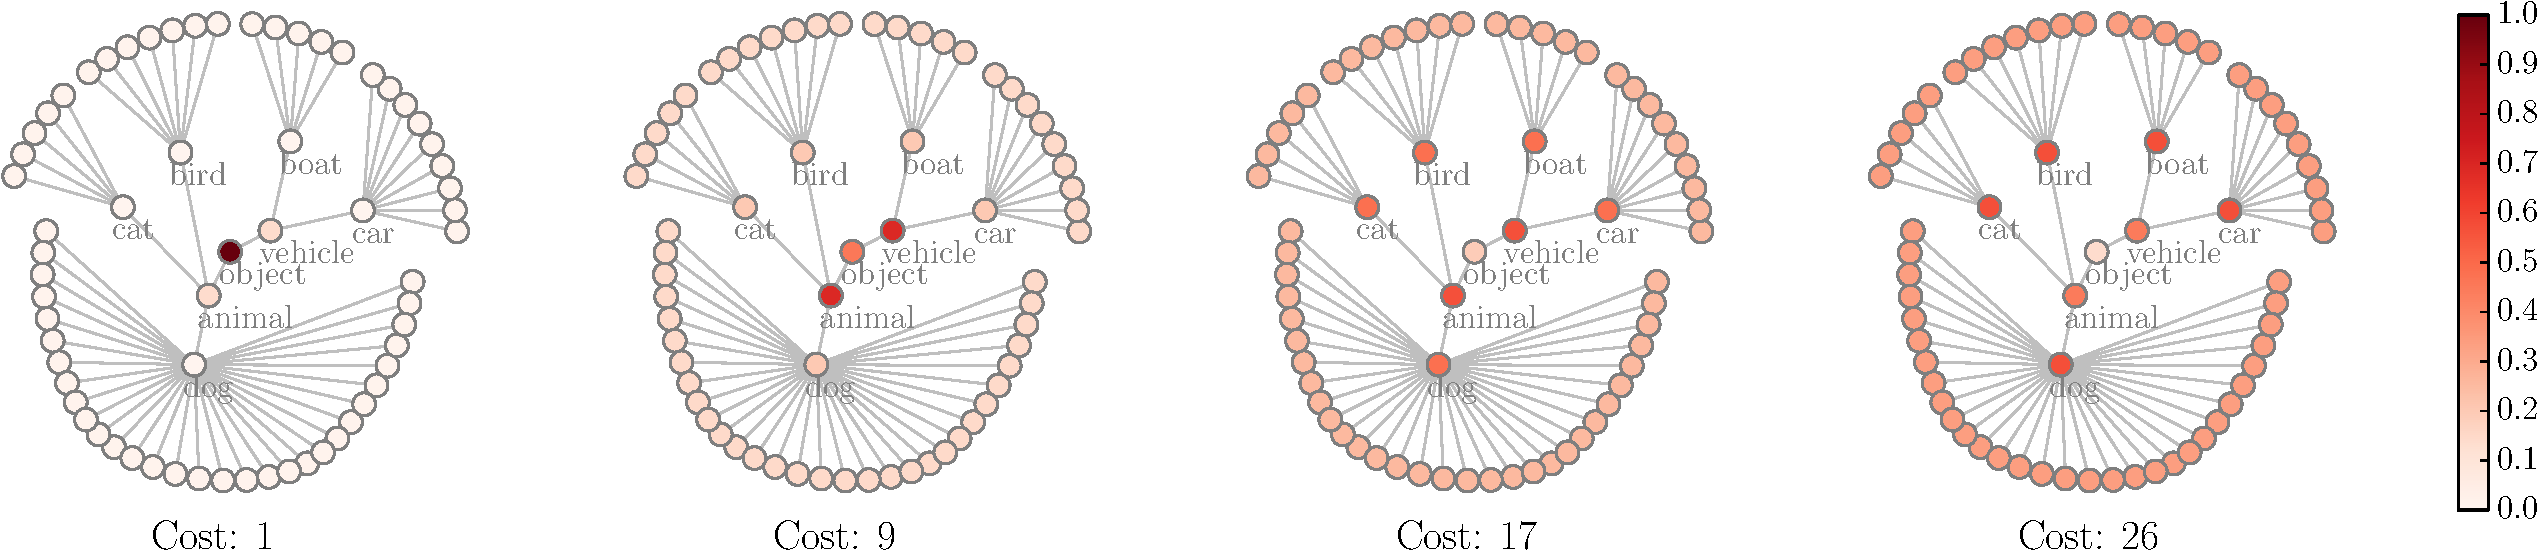
\includegraphics[width=\textwidth]{../../figures/apr11_assembly/ilsvrc65_network-crop.pdf}
            \caption{
            We visualize the fraction of predictions made at inner vs. leaf nodes of ILSVRC-65 at different cost points of an Anytime policy: with more computation, accurate predictions are increasingly made at the leaf nodes.
            \label{fig:imagenet-c}
            }
    \end{subfigure}
\caption{
Results on the ILSVRC-65 dataset (best viewed in color).
Figure (a) shows our dynamic approaches outperforming static baselines for all practical cost budgets.
When our method is combined with Hedging Your Bets \parencite{Deng-CVPR-2012}, a constant prediction accuracy can be achieved at all points in the Anytime policy, with \emph{specificity} of predictions increasing with the cost of predictions.
Figures (b) and (c) show this for the \emph{dynamic, non-myopic} policy learned for budget = 26.
This is analogous to human visual performance, which shows increased specificity at longer stimulus times.
}\label{fig:imagenet}
\end{figure*}


\PM{Setup}
The full ImageNet dataset has over 10K categories and over a million images \parencite{Deng-ECCV-2010}.
The classes are organized in a hierarchical structure, which can be exploited for novel recognition tasks.
We evaluate on a 65-class subset introduced in ``Hedging Your Bets'' \parencite{Deng-CVPR-2012}.
In this evaluation, we consider the situation where the initial feature computation has already happened, and the task is to find a path through existing one-vs-all classifiers: features correspond to Platt-scaled SVM confidences of leaf-node classifiers (trained on SIFT-LLC features), and each has cost 1 \parencite{Deng-ECCV-2010}.
Following \parencite{Deng-CVPR-2012}, accuracy is defined on all nodes, and inner node confidences are obtained by summing the probabilities of the descendant nodes.

\PM{Results}
We combine our sequential feature selection with the ``Hedging Your Bets'' method for backing off prediction nodes using the ImageNet hierarchy to maintain guaranteed accuracy while giving maximally specific answers, given a cost budget.
The results are given in \autoref{fig:imagenet}.
As the available budget increases, the \emph{specificity} (defined by normalized information gain in the hierarchy) of our predictions also increases, while accuracy remains constant.
Visualizing this on the ILSVRC-65 hierarchy, we see that the fraction of predictions at the leaf nodes grows with available computation time.
This formulation presents a novel angle on modeling the time course of human visual perception.

